\documentclass{beamer}
\usetheme{Madrid}

\usepackage{amsmath}
\usepackage{graphicx}
% \usepackage{multicol}
% \usepackage{multirow}

\usepackage{tikz}
\usetikzlibrary{shapes.geometric, arrows}
% \usepackage{pgfplots}

\usepackage[justification=centering]{caption}
\usepackage{subcaption}

\usepackage{xurl}

% default path to images and other assets
\graphicspath{{../assets/}}

% disable wrapping
\tolerance=1
\emergencystretch=\maxdimen
\hyphenpenalty=10000
\hbadness=10000

% number figure caption
\setbeamertemplate{caption}[numbered]

% display bib label in references
\setbeamertemplate{bibliography item}{\insertbiblabel}
\setbeamertemplate{bibliography entry title}{}
\setbeamertemplate{bibliography entry location}{}
\setbeamertemplate{bibliography entry note}{}

% Metadata
% ------------------------
\title[MultiCut GNN]{Graph neural network for solving the minimum cost multicut problem}
\subtitle{Research seminar combinatorial image analysis}

\author{Oleh Shkalikov}

\institute[TU Dresden]{TU Dresden, Computer Science Faculty}

\date{13 June, 2023}

% ------------------------


\tikzstyle{main_node} = [circle, minimum width=1cm,text centered, draw=black, fill=red!30]
\tikzstyle{neigh_node} = [circle, minimum width=1cm,text centered, draw=black, fill=green!30]
\tikzstyle{node} = [circle, minimum width=1cm,text centered, draw=black, fill=cyan!30]
\tikzstyle{arrow} = [thick,->,>=stealth]

\begin{document}

\frame{\titlepage}

\begin{frame}
    \frametitle{Agenda}
    \tableofcontents
\end{frame}

\section{The multicut problem and introduction to GNN}

\begin{frame}
    \frametitle{Minimum Cost MultiCut Problem}

    For the given graph $G = (V, E)$ and an associated cost
    function $w: E \to \mathbb{R}$, the multicut problem is

    \begin{alignat*}{2}
        \min_{y \in \{0, 1\}^E} \quad &
        c(y) = \sum\limits_{e \in E} w_e y_e                                            \\
        \text{subject to:}      \quad &
        y_e \leq \sum\limits_{e' \in C \setminus \{e\}} y_{e'}                          \\
                                      & \forall C \in \text{cycles}(G), \forall e \in C
    \end{alignat*}

    \begin{alertblock}{Complexity}
        The problem of finding the optimal solution for this ILP
        is NP-hard problem. Moreover, the number of constraints grows
        exponentially.
    \end{alertblock}

\end{frame}

\begin{frame}
    \frametitle{Graph Neural Network}

    For the given update function $\gamma$, message $\phi$, and
    commutative aggregation operation $\bigotimes$, the update rule for every
    node $i$ at step $t$ with node feature vector $\mathbf{x}$ and
    edge feature vector $\mathbf{e}$ (optional) is
    \[
        \mathbf{x}_i^{(t+1)} = \gamma^{(t)} \left(\mathbf{x}_i^{(t)},
        \bigotimes_{j \in \mathcal{N}(i)} \phi^{(t)} \left(\mathbf{x}^{(t)}_i,
        \mathbf{x}^{(t)}_j, \mathbf{e^{(t)}}_{j, i} \right) \right)
    \]

    \begin{figure}
        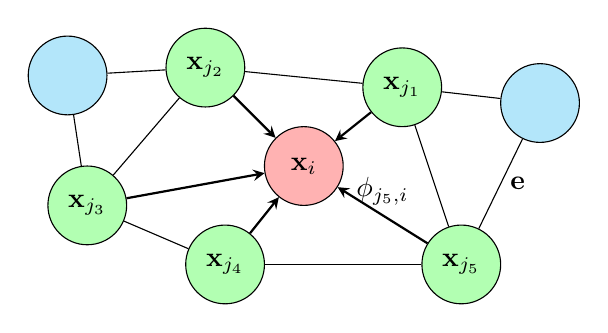
\begin{tikzpicture}[node distance=1.25cm]
            \node(main) [main_node] {$\mathbf{x}_i$};
            \node(neigh1) [neigh_node, right of=main, yshift=1cm] {$\mathbf{x}_{j_1}$};
            \node(neigh2) [neigh_node, left of=main, yshift=1.25cm] {$\mathbf{x}_{j_2}$};
            \node(neigh3) [neigh_node, left of=main, xshift=-1.5cm, yshift=-0.5cm] {$\mathbf{x}_{j_3}$};
            \node(neigh4) [neigh_node, below of=main, xshift=-1cm] {$\mathbf{x}_{j_4}$};
            \node(neigh5) [neigh_node, below of=main, xshift=2cm] {$\mathbf{x}_{j_5}$};

            \node(node1) [node, right of=neigh1, xshift=0.5cm, yshift=-0.2cm] {};
            \node(node2) [node, left of=neigh2, xshift=-0.5cm, yshift=-0.1cm] {};

            \draw[arrow] (neigh1) -- (main);
            \draw[arrow] (neigh2) -- (main);
            \draw[arrow] (neigh3) -- (main);
            \draw[arrow] (neigh4) -- (main);
            \draw[arrow] (neigh5) -- node[above]{$\phi_{j_5, i}$} (main);

            \draw (neigh1) -- (neigh2);
            \draw (neigh1) -- (neigh5);
            \draw (neigh2) -- (neigh3);
            \draw (neigh3) -- (neigh4);
            \draw (neigh4) -- (neigh5);
            \draw (neigh1) -- (node1);
            \draw (neigh5) -- node[right]{$\mathbf{e}$} (node1);
            \draw (neigh2) -- (node2);
            \draw (neigh3) -- (node2);
        \end{tikzpicture}
        \caption{Illustration of the message passing scheme}
    \end{figure}

\end{frame}

\begin{frame}
    \frametitle{Laplacian and Discrete Fourier Transform}
    The discrete fourier transform can be represented as a matrix:
    \[
        U = \begin{pmatrix}
            u_0(0)   & u_1(0)   & \dots  & u_{N-1}(0)   \\
            u_0(1)   & u_1(1)   & \dots  & u_{N-1}(1)   \\
            \vdots   & \vdots   & \ddots & \vdots       \\
            u_0(N-1) & u_1(N-1) & \dots  & u_{N-1}(N-1)
        \end{pmatrix}
    \]
    where
    \[
        u_n(x) = \cos\left(2 \pi \frac{n}{N} x \right) -
        i \sin\left(2 \pi \frac{n}{N} x \right)
    \]

    At the same time these $u_n$ are eigenvectors of the
    Laplacian operator:
    \[
        \Delta u_n(x) = \left( -4 \pi \frac{n^2}{N^2} \right) u_n(x)
    \]

\end{frame}

\begin{frame}
    \frametitle{Graph Convolutional Network}

    For the given adjacency matrix $A$ and degree matrix $D$ the
    graph laplacian is the following:
    \[
        L = I_N - D^{-\frac{1}{2}} A D^{-\frac{1}{2}} = U \Lambda U^T
    \]

    Thus, the convolution can be computed:
    \[
        g_{\theta} \star \mathbf{x} = U \hat{g}_{\theta} U^T \mathbf{x}
    \]

    Approximated form \cite{kipf2016semi} after renormalization trick as a message passing:
    \[
        \mathbf{x}_i^{(t+1)} =
        \sum_{j \in \mathcal{N}(i) \cup \{ i \}}
        \frac{\theta \mathbf{x}_j^{(t)}}
        {\sqrt{\deg(i)} \sqrt{(\deg(j))}}
    \]

\end{frame}

\section{GNN approaches for multicuts}

\subsection{Supervised learning}

\begin{frame}
    \frametitle{GNN MultiCut Pipeline}



\end{frame}

\begin{frame}
    \frametitle{Edge-Weighted GCN}



\end{frame}

\begin{frame}
    \frametitle{Evaluation Results}



\end{frame}

\begin{frame}
    \frametitle{Scaling Study}



\end{frame}

\begin{frame}
    \frametitle{Learning Node Embedding: Motivation}



\end{frame}

\begin{frame}
    \frametitle{Learning Node Embedding}



\end{frame}

\begin{frame}
    \frametitle{Relaxed Cycle Consistency Loss}

\end{frame}

\begin{frame}
    \frametitle{Edge Weight Embedding}



\end{frame}

\subsection{Unsupervised learning}

\begin{frame}
    \frametitle{MultiCut Cost Loss}

\end{frame}

\subsection{Self-prior learning}

\begin{frame}
    \frametitle{Overfit Is All You Need}



\end{frame}

\section*{References}

\begin{frame}[allowframebreaks]
    \frametitle{References}

    \bibliographystyle{apalike}
    \bibliography{../references.bib}
\end{frame}

\end{document}